\documentclass[a4paper]{scrartcl}
\usepackage[
    typ=ueb,
    klausurtyp=kurs,
    klasse=scrartcl,
    fach=LF05 Physik,
    lerngruppe=T20E,
    loesungen=seite,
    module={Symbole,Bewertung}    
    %erwartungshorizontAnzeigen,
    %erwartungshorizontStil=simpel,
hHh]{schule}
% Dieses Dokument gehört zu den Beispiel des LaTeX Paketes Schule und ist von den Autoren
% des Pakets erstellt worden.
%
% Das Dokument steht unter der Lizenz: Creative Commons by-nc-sa Version 4.0
% http://creativecommons.org/licenses/by-nc-sa/4.0/deed.de
%
% Nach dieser Lizenz darf das Dokument beliebig kopiert und bearbeitet werden,
% sofern das Folgeprodukt wiederum unter gleichen Lizenzbedingungen vertrieben
% und auf die ursprünglichen Urheber verwiesen wird.
% Eine kommerzielle Nutzung ist ausdrücklich ausgeschlossen.

\author{Heiko Schröter}
\date{\today}
\title{Wärmelehre\\
(Ausdehnung und innere Energie)}
\subtitle{Übungsaufgaben zur Ausdehnung und innere Energie}

\usepackage{amsmath}
\usepackage{pgfplots}
\usepackage{mathrsfs}
\usepackage{xfrac}
\usepackage{siunitx}
%\sisetup{quotient-mode = fraction, locale = DE}
\sisetup{per-mode = fraction, locale = DE}
\usepackage{blindtext}
\usepackage{enumitem}
\newcommand{\Ergebnis}[1]{\underline{\underline{#1}}}
\usepackage{graphicx}
\usepackage{hyperref}
\usepackage{xltabular}
\renewcommand{\labelenumi}{\alph{enumi})}

\begin{document}
\sffamily
\begin{aufgabe}[points={2}]
Ein Stahlkugel hat einen Durchmesser von $\SI{10}{\centi\meter}$ und wird um $\SI{300}{\celsius}$ erwärmt. Welchen Raum nimmt sie dann ein, wenn mit einer \glqq mittleren\grqq \quad Wärmedehnzahl $\alpha=\SI{0,000012}{\meter\per\meter\per\kelvin}$ gerechnet wird?\\
	
\begin{tikzpicture}
		\draw[step=0.5cm,gray,very thin] (0,0) grid (16.5,4);
	\end{tikzpicture}
	
    \begin{loesung}
    \begin{flalign*}
	V_2&=V_1+V_1\cdot\gamma\cdot\Delta\vartheta=V_1+V_1\cdot 3\alpha\cdot\Delta\vartheta\\
	V_1&=\dfrac{\pi}{6}\cdot d^{3}=\dfrac{\pi}{6}\cdot (\SI{10}{\centi\meter})^{3}=\SI{523,599}{\cubic\centi\meter}\\
	V_2&=\SI{523,599}{\cubic\centi\meter}+\SI{523,599}{\cubic\centi\meter}\cdot 3\cdot\SI{0,000012}{\meter\per\meter\per\kelvin}\cdot\SI{300}{\kelvin}\\
	&=\SI{523,599}{\cubic\centi\meter}+\SI{5,655}{\cubic\centi\meter}=\Ergebnis{\SI{529,254}{\cubic\centi\meter}}&
	\end{flalign*}
    \end{loesung}
\end{aufgabe}

\begin{aufgabe}[points={7}]
    Über der Mitte einer \SI{20}{\meter} breiten Straße ist eine Lampe an einem Stahlseil aufgehängt. Der Durchhang soll bei \SI{-20}{\celsius} \SI{0,4}{\meter} betragen. ($\alpha_{Stahl}=\SI{11,5e-6}{\per\kelvin}$)\\
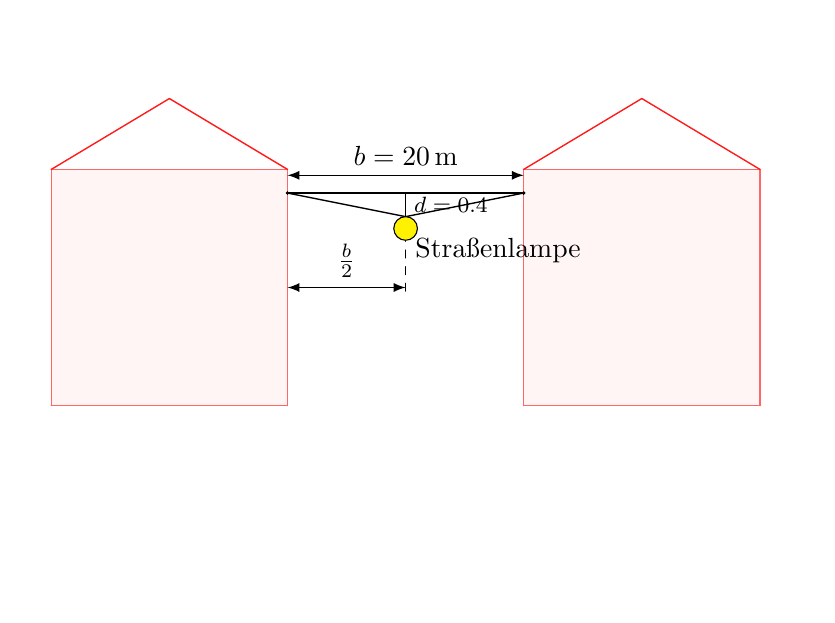
\begin{tikzpicture}[scale=0.15, line cap=round]
%\begin{tikzpicture}[scale=0.6, line cap=round,line join=round,>=triangle 45,x=0.3cm,y=0.3cm]
\clip(-22.,-16.) rectangle (44.,32.);
\fill[line width=1.pt,color=red!40!white,fill=red!40!white,fill opacity=0.1] (0.,0.) -- (0.,20.) -- (-20.,20.) -- (-20.,0.) -- cycle;
\fill[line width=1.pt,color=red!40!white,fill=red!40!white,fill opacity=0.1] (40.,0.) -- (40.,20.) -- (20.,20.) -- (20.,0.) -- cycle;
\draw [line width=0.5 pt,color=red!60!white] (0.,0.)-- (0.,20.);
\draw [line width=0.5 pt,color=red!60!white] (0.,20.)-- (-20.,20.);
\draw [line width=0.5 pt,color=red!60!white] (-20.,20.)-- (-20.,0.);
\draw [line width=0.5 pt,color=red!60!white] (-20.,0.)-- (0.,0.);
\draw [line width=0.5 pt,color=red!60!white] (40.,0.)-- (40.,20.);
\draw [line width=0.5 pt,color=red!60!white] (40.,20.)-- (20.,20.);
\draw [line width=0.5 pt,color=red!60!white] (20.,20.)-- (20.,0.);
\draw [line width=0.5 pt,color=red!60!white] (20.,0.)-- (40.,0.);
\draw [line width=0.5 pt,color=red!90!white] (-20.,20.)-- (-10.,26.);
\draw [line width=0.5 pt,color=red!90!white] (-10.,26.)-- (0.,20.);
\draw [line width=0.5 pt,color=red!90!white] (20.,20.)-- (30.,26.);
\draw [line width=0.5 pt,color=red!90!white] (30.,26.)-- (40.,20.);
\draw [thick] (0.,18.)-- (20.,18.);
\filldraw[fill=white, draw=black] (0.,18.) circle (0.1cm);
\filldraw[fill=white, draw=black] (20.,18.) circle (0.1cm);
\draw [<->, >=latex, line width=0.5 pt] (0.,19.5)-- (20.,19.5) node [above, midway] {$b = \SI{20}{\meter}$};
{\footnotesize \draw [line width=0.5 pt] (10.,18.)-- (10.,16.) node [right, midway] {$d = 0.4$};}
\draw [<->, >=latex, line width=0.5 pt] (0.,10)-- (10.,10) node [above, midway] {$\frac{b}{2}$};
\draw [line width=0.5 pt] (10.,16.)-- (20.,18.);
\draw [line width=0.5 pt] (0.,18.)-- (10.,16.);
\draw [very thin, dashed] (10.,16.)-- (10.,9.5);
\filldraw[fill=yellow, draw=black] (10.,15.0) circle (1cm) node [anchor=north west] {Straßenlampe};
\begin{scriptsize}
\end{scriptsize}
\end{tikzpicture}
    \begin{teilaufgaben}
        \teilaufgabe Welche Seillänge muss bei \SI{22}{\celsius} verlegt werden?
        \teilaufgabe Wie groß ist der Durchhang bei \SI{32}{\celsius}?
    \end{teilaufgaben}
	
\begin{tikzpicture}
		\draw[step=0.5cm,gray,very thin] (0,0) grid (16.5,4);
	\end{tikzpicture}
    \begin{loesung}
    Seillänge bei \SI{-20}{\celsius}:
\begin{flalign*}
\dfrac{l_1}{2}=\sqrt{\left(\dfrac{b}{2}\right)^{2}+d^{2}}=\sqrt{\left(\dfrac{\SI{20}{\meter}}{2}\right)^{2}+(\SI{0,4}{\meter})^{2}}=\SI{10,008}{\meter}\Rightarrow l_1=\SI{20,016}{\meter}&
\end{flalign*}
        \begin{teilaufgaben}
            \teilaufgabe
Seillänge bei \SI{22}{\celsius}:
\begin{flalign*}
&l_2=l_1(1+\alpha\Delta\vartheta)=\SI{20,016}{\meter}\left(1+\SI{11,5e-6}{\per\kelvin}\cdot\SI{42}{\kelvin}\right)=\Ergebnis{\SI{20,026}{\meter}}&
\end{flalign*}           
            \teilaufgabe 
Durchhang bei \SI{32}{\celsius}
\begin{flalign*}
l_3&=l_1(1+\alpha\Delta\vartheta)=\SI{20,016}{\meter}\left(1+\SI{11,5e-6}{\per\kelvin}\cdot\SI{52}{\kelvin}\right)=\SI{20,028}{\meter}\\
d_3&=\sqrt{\left(\dfrac{l_3}{2}\right)^{2}-\left(\dfrac{b}{2}\right)^{2}}=\sqrt{\left(\dfrac{\SI{20,028}{\meter}}{2}\right)^{2}-\left(\dfrac{\SI{20}{\meter}}{2}\right)^{2}}=\Ergebnis{\SI{0,529}{\meter}}&
\end{flalign*} 
        \end{teilaufgaben}
    \end{loesung}
\end{aufgabe}
\vspace{1cm}

\begin{aufgabe}[points={6}]
	Ein Benzintank mit \SI{20}{\liter} Volumen wird bei \SI{12}{\celsius} mit \SI{19,5}{\liter} Benzin gefüllt. Bei welcher Temperatur läuft das Benzin über, wenn der Tank aus Stahlblech besteht? ($\alpha_{Stahl}=\SI{11,5e-6}{\per\kelvin}$, $\gamma_{Benzin}=\SI{10e-4}{\per\kelvin}$)\\
	
\begin{tikzpicture}
		\draw[step=0.5cm,gray,very thin] (0,0) grid (16.5,4);
	\end{tikzpicture}        
        \begin{loesung}
\begin{flalign*}
V_{B2}&=V_{B1}(1+\gamma\Delta\vartheta)=\SI{19,5}{\liter}\cdot\left(1+\SI{10e-4}{\per\kelvin}\cdot\Delta\vartheta\right)\\
V_{T2}&=V_{T1}(1+\num{3}\alpha\Delta\vartheta)=\SI{20}{\liter}\cdot\left(1+\num{3}\cdot\SI{11,5e-6}{\per\kelvin}\cdot\Delta\vartheta\right)\\
V_{B2}&=V_{T2}\Rightarrow \SI{19,5}{\liter}\cdot\left(1+\SI{10e-4}{\per\kelvin}\cdot\Delta\vartheta\right)=\SI{20}{\liter}\cdot\left(1+\num{3}\cdot\SI{11,5e-6}{\per\kelvin}\cdot\Delta\vartheta\right)\\
\SI{19,5}{\liter}&+\SI{19,5}{\liter}\cdot\SI{10e-4}{\per\kelvin}\cdot\Delta\vartheta=\SI{20}{\liter}+\SI{20}{\liter}\cdot\num{3}\cdot\SI{11,5e-6}{\per\kelvin}\cdot\Delta\vartheta\\
\SI{19,5}{\liter}&-\SI{20}{\liter}=\SI{20}{\liter}\cdot\num{3}\cdot\SI{11,5e-6}{\per\kelvin}\cdot\Delta\vartheta-\SI{19,5}{\liter}\cdot\SI{10e-4}{\per\kelvin}\cdot\Delta\vartheta\\
\SI{19,5}{\liter}&-\SI{20}{\liter}=\Delta\vartheta\cdot\left(\SI{20}{\liter}\cdot\num{3}\cdot\SI{11,5e-6}{\per\kelvin}-\SI{19,5}{\liter}\cdot\SI{10e-4}{\per\kelvin}\right)\\
\Delta\vartheta &=\dfrac{\SI{19,5}{\liter}-\SI{20}{\liter}}{\left(\SI{20}{\liter}\cdot\num{3}\cdot\SI{11,5e-6}{\per\kelvin}-\SI{19,5}{\liter}\cdot\SI{10e-4}{\per\kelvin}\right)}=\SI {26,6}{\kelvin}\\
\vartheta_2&=\vartheta_1+\Delta\vartheta=\SI{12}{\celsius}+\SI{26,6}{\kelvin}=\Ergebnis{\SI{38,6}{\celsius}}&
\end{flalign*}
    	\end{loesung}
\end{aufgabe}
\vspace{1cm}

\begin{aufgabe}[points={3}]
	Welche Wärmemenge ist erforderlich, um \SI{80}{\liter} Wasser von \SI{14}{\celsius} auf \SI{85}{\celsius} zu erwärmen?\\
	
\begin{tikzpicture}
		\draw[step=0.5cm,gray,very thin] (0,0) grid (16.5,4);
	\end{tikzpicture}       
        \begin{loesung}
\begin{flalign*}
&Q=c\cdot m\Delta\vartheta=\SI{4,187}{\kilo\joule\per\kilogram\per\kelvin}\cdot\SI{80}{\kilogram}\cdot\SI{71}{\kelvin}=\Ergebnis{\SI{23,8}{\mega\joule}}&
\end{flalign*} 
    	\end{loesung}
\end{aufgabe}

\begin{aufgabe}[points={3}]
	Das Gehäuse eines Transistors hat eine Wärmekapazität von \SI{27}{\joule\per\kelvin}. Durch einen Stromimpuls wird dem Transistor die Wärme \SI{100}{\joule} zugeführt. Um wie viel Kelvin steigt die Gehäusetemperatur an? Hinweis: Wärmekapazität des Kristalls bleibt unberücksichtigt.\\
	
\begin{tikzpicture}
		\draw[step=0.5cm,gray,very thin] (0,0) grid (16.5,4);
	\end{tikzpicture}        
        \begin{loesung}
\begin{flalign*}
&Q=C\Delta\vartheta\Rightarrow \Delta\vartheta=\dfrac{Q}{C}=\dfrac{\SI{100}{\joule}}{\SI{27}{\joule\per\kelvin}}=\Ergebnis{\SI{3,7}{\kelvin}}&
\end{flalign*} 
    	\end{loesung}
\end{aufgabe}
\vspace{0.5cm}
\newline
\end{document}